% ********** Rozdział 2 **********
\chapter{Opis struktury projektu}

Projekt składa się z kilku części: Klasy główne(Models), Klasy używane do nawigacji, Komendy, Klasa do przechowywania ViewModels(NavigateStore) i Klasa do wykorzystania bazy danych. Klasy główne używane są do przechowywania danych z bazy(np. Pracownik lub Wizyta). Klasy nawigacyjne używane są do przechowywania danych i operacji nad danymi pobranych od użytkownika w widoku(View) lub z bazy danych(np. UserInfoViewModel przechowuje informacje pobraną z bazy danych i przenosi ją do UserInfoView). Komendy wykorzystane są do nawigacji, przesłania danych do bazy danych lub otrzymania danych.

\section{Diagram klas}

\begin{figure}[H]
\begin{center}
    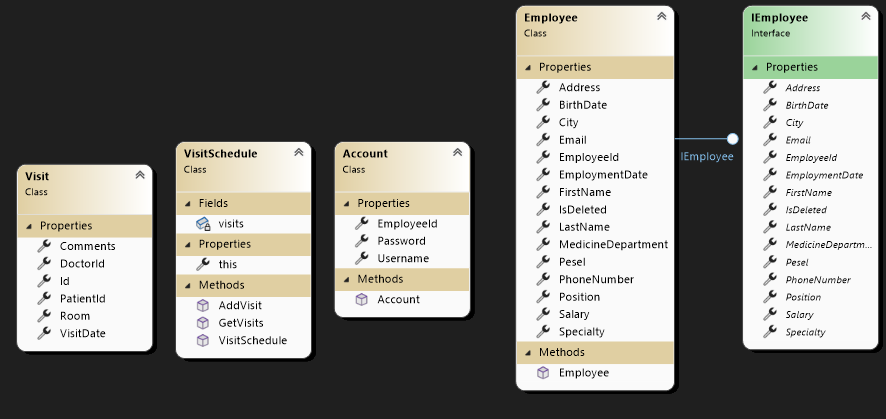
\includegraphics[height=8cm]{images/diag_gl_kl.png}
    \caption{Klasy główne}
\end{center}
\end{figure}

\begin{figure}[H]
\begin{center}
    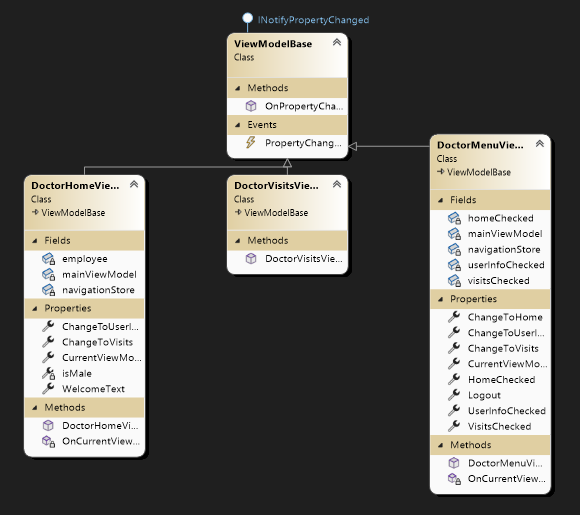
\includegraphics[height=10cm]{images/diag_kl_nav_dok.png}
    \caption{Klasy nawigacyjne dla doktora}
\end{center}
\end{figure}

\begin{figure}[H]
\begin{center}
    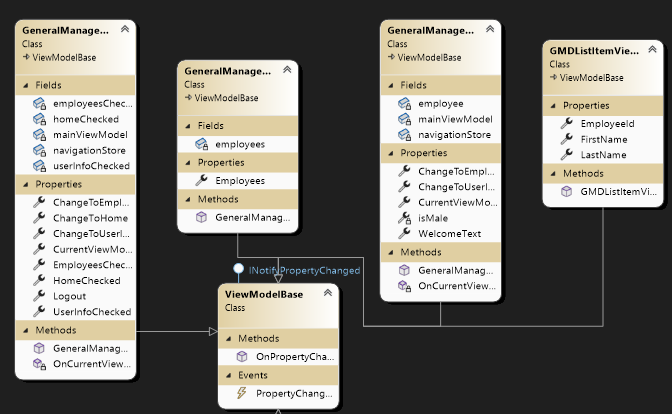
\includegraphics[height=10cm]{images/diag_kl_nav_gen_man.png}
    \caption{Klasy nawigacyjne dla głównego kierownika}
\end{center}
\end{figure}

\begin{figure}[H]
\begin{center}
    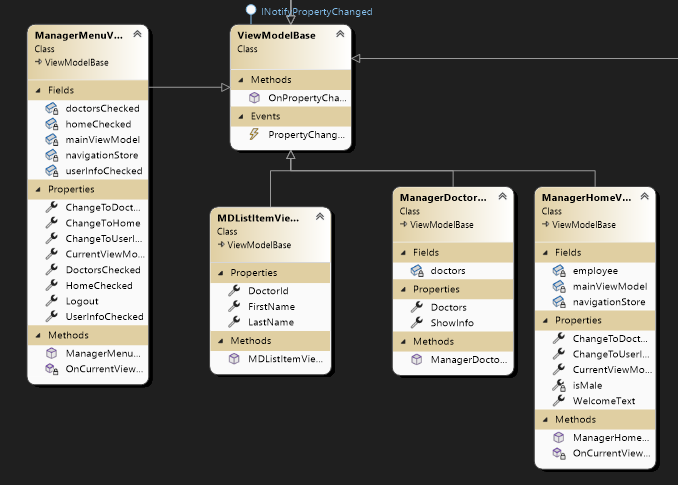
\includegraphics[height=10cm]{images/diag_kl_nav_mang.png}
    \caption{Klasy nawigacyjne dla kierownika}
\end{center}
\end{figure}

\begin{figure}[H]
\begin{center}
    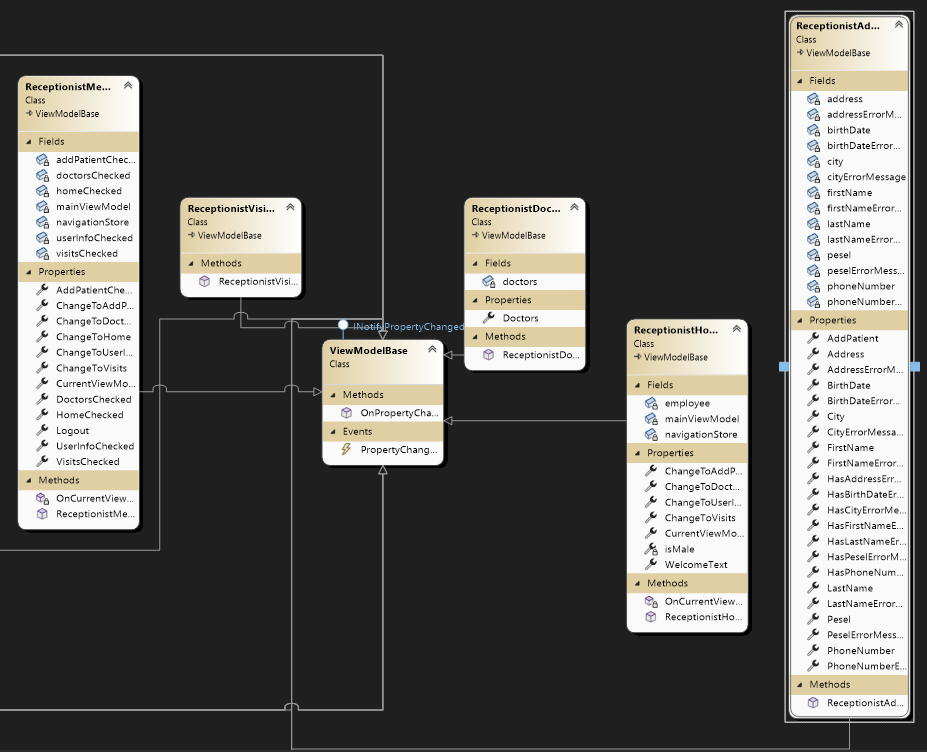
\includegraphics[height=10cm]{images/diag_kl_nav_recep.png}
    \caption{Klasy nawigacyjne dla recepcjonisty}
\end{center}
\end{figure}

\begin{figure}[H]
\begin{center}
    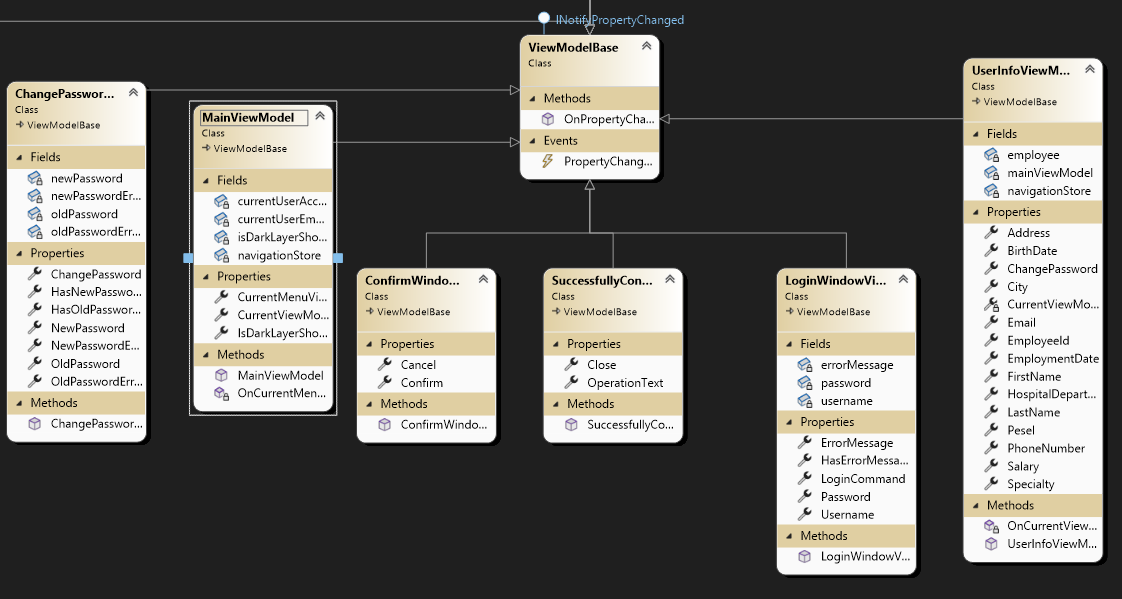
\includegraphics[height=9cm]{images/diag_kl_nav_wszt.png}
    \caption{Klasy nawigacyjne wspólne dla wszystkich klientów}
\end{center}
\end{figure}

\begin{figure}[H]
\begin{center}
    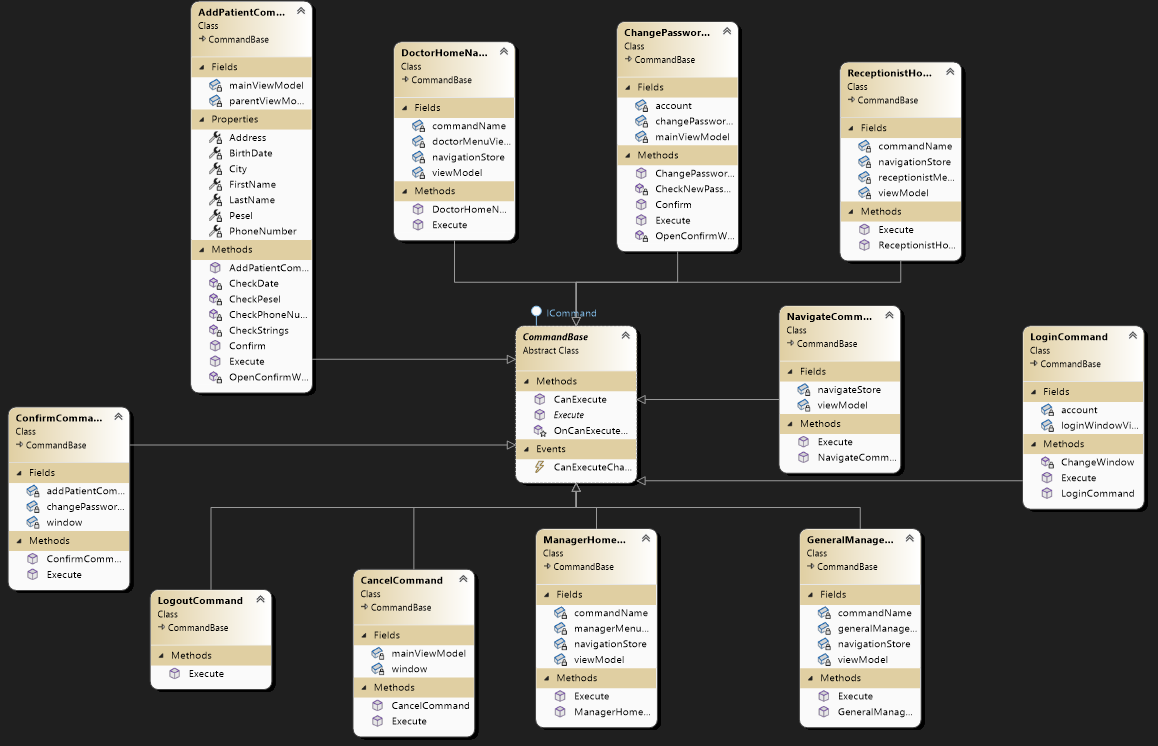
\includegraphics[height=10cm]{images/diag_kl_kom.png}
    \caption{Klasy komend}
\end{center}
\end{figure}

\begin{figure}[H]
\begin{center}
    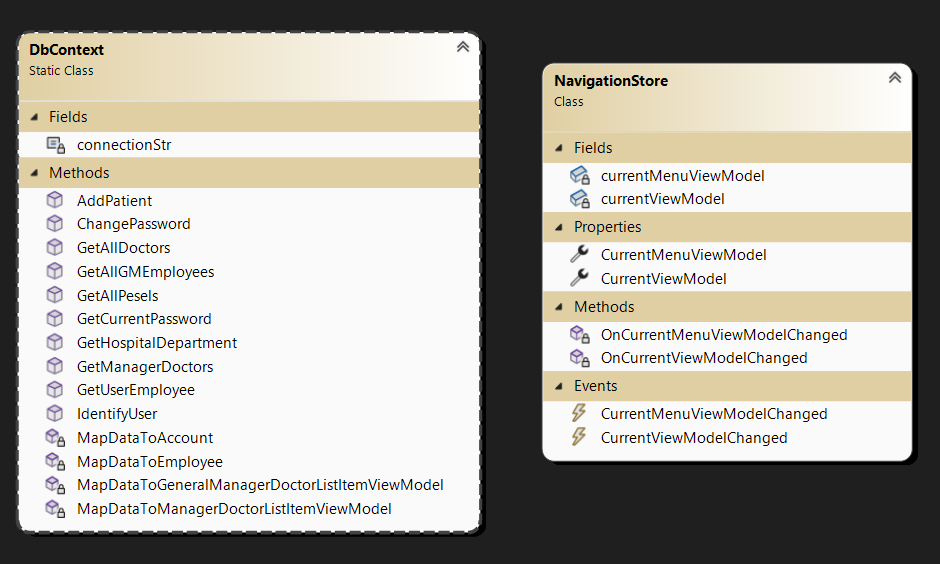
\includegraphics[height=8cm]{images/diag_kl_db_nav.png}
    \caption{Klasy dla bazy danych i przechowywania nawigacji}
\end{center}
\end{figure}

\section{Narzędzie}

Do tworzenia aplikacji \textquotedbl Szpital+\textquotedbl{} korzystałem z narzędzi {\color{blue}\href{https://pl.wikipedia.org/wiki/Windows_Presentation_Foundation}{WPF(Windows Presentation Foundation)}}. Jest to narzędznie do trowrzenia aplikacji desktopowych dla systemów Windows na bazie {\color{blue}\href{https://pl.wikipedia.org/wiki/.NET_Framework}{.Net Framework}}. Wykorzystywuje język opisy interfejsu użytkownika({\color{blue}\href{https://pl.wikipedia.org/wiki/Extensible_Application_Markup_Language}{XAML}}\label{href:XAML}) oraz język programowania {\color{blue}\href{https://pl.wikipedia.org/wiki/C_Sharp}{C\#}}\label{href:c_sh} do implementacji funkcjonalności elementów i innych funckji backend. 

Dodatkowo przestrzegałem {\color{blue}\href{https://en.wikipedia.org/wiki/Model%E2%80%93view%E2%80%93viewmodel}{wzóru architektonicznego MVVM}}(Model-View-ViewModel)\label{href:MVVM}. Jest to wzór który rozdziela graficzny interfejs użytkownika GUI(View) od implementacji logiki biznesowej oraz logiki backend. Związkiem między tymi warstami jest konwerter wartości (ViewModel), który przyjmuje publiczne właściwości modeli(Models) i przekazuje ich do widoków(Views) za pomocą wiązania (Binding).

Do pisania kodu korzystałem z środowiska programistycznego {\color{blue}\href{https://pl.wikipedia.org/wiki/Microsoft_Visual_Studio}{Microsoft Visual Studio}\label{href:VStudio}}.

Także wykorzystełem wtyczki \textquotedbl {\color{blue} \href{https://github.com/charri/Font-Awesome-WPF}{FontAwesome.WPF}}\textquotedbl{} dla dodania ikon jako tekstu dla nawigacji bocznej i wtyczki \textquotedbl {\color{blue}\href{https://github.com/dotnet/corefx}{System.Data.SqlClient}}\textquotedbl{} dla połączenia z bazą danych SQL.

\newpage

\section{Baza danych}

Do stworzenia i zarządzania bazą danych wykorzystywałem {\color{blue}\href{https://en.wikipedia.org/wiki/SQL_Server_Management_Studio}{Microsoft SQL Server Management Studio}}. Na lokalnym serwerze stworzyłem bazę danych "Spzital". Także uzupełniłem bazę losowymi wartościami i dodałem kilka ograniczeń. Na przykład ograniczenie na wprowadzenie do nr\_gabinetu w wizycie większego od 127.

\begin{figure}[H]
\begin{center}
    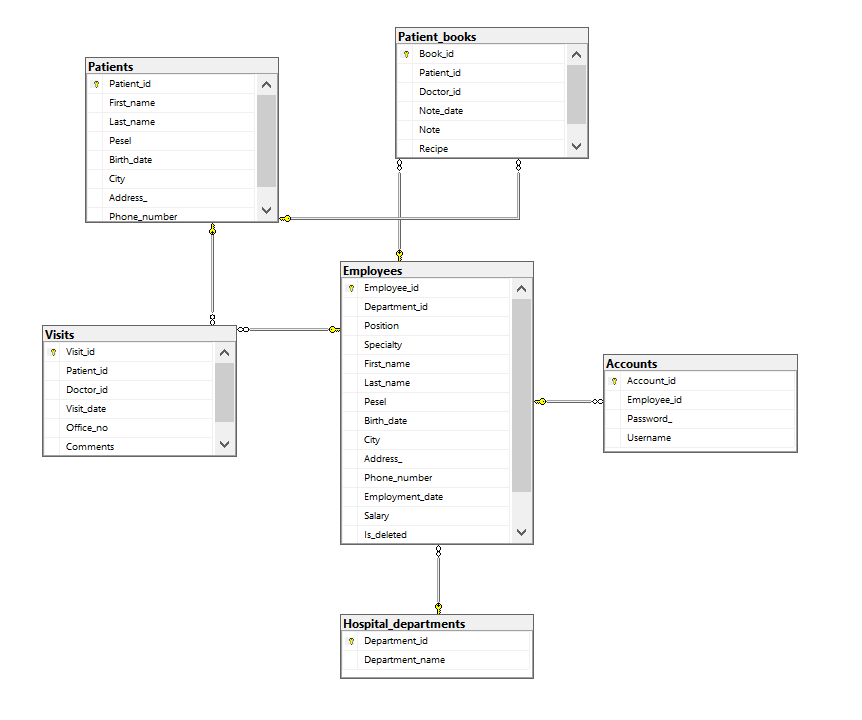
\includegraphics[height=12cm]{images/db_diagram.png}
    \caption{Diagram bazy danych}
\end{center}
\end{figure}

Do pobrania danych z bazy do aplikacji wykorzystuję klasy statycznej DbContext w której są metody robiące zapytania na bazę danych i wracające wartości pobrane z bazy.

\begin{figure}[H]
    \centering
    \subfigure{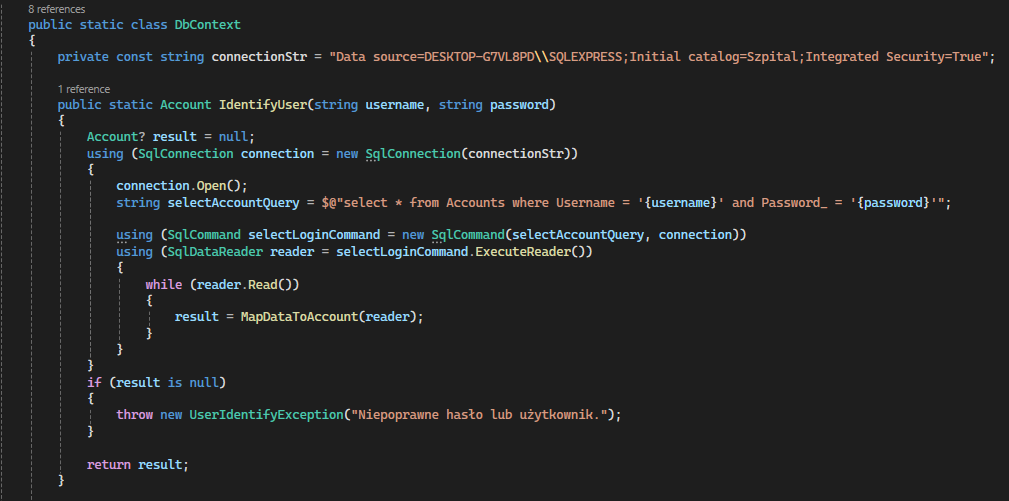
\includegraphics[width=0.7\textwidth]{images/db_cont_klas1.png}} 
    \subfigure{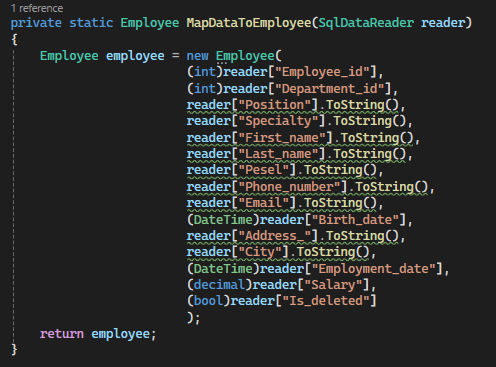
\includegraphics[width=0.7\textwidth]{images/db_cont_klas2.png}} 
    \caption{Klasa do zarządzania bazą danych(Przykładowa metoda)}
\end{figure}

\section{Minimalne wymagania sprzętowe}
\begin{itemize}
    \item System operacyjny: Microsoft Windows 10 lub wyżej
    \item Procesor: x86 lub x64 z szybkością > 800 MHz
    \item RAM: 512 MB
    \item Miejsca na dysku: 25 MB
    \item Zainstalowany .Net 8.0
\end{itemize}


% ********** Koniec rozdziału **********
